\documentclass[10pt,a4paper]{article}

\usepackage[utf8]{inputenc}
\usepackage{graphicx}
\usepackage{textcomp}
\usepackage{booktabs}
\usepackage{subcaption}
\usepackage{comment}
\usepackage[hmargin=2.5cm,vmargin=2.5cm,bindingoffset=0.5cm]{geometry}

\title{Pattern Classification and Machine Learning\\\Huge Miniproject}
\author{Taha Elgraini (SCIPER ID: 238189), Fabian Brix (SCIPER ID: 236334)\\Group 22, Python}

\begin{document}

\maketitle

\section{Introduction}
The imperative of this project was to apply two different machine learning techniques, the Multilayer Perceptron (henceforth referred to as "MLP") and the Support Vector Machine (henceforth "SVM") to the recognition of hand-written digits. More specifically error back-propagation gradient descent optimization had to be implemented for MLP and the Sequential Minimal Optimization (SMO) algorithm had to be implemented for SVM to solve problems posed with th0,00140e MNIST dataset. The MLP had to be trained on datasets of digits 3 and 5 as well as of 4 and 5, whereas the SVM classifier only had to be trained on the 3/5 problem. Both classifiers should accurately classify the digits in a test set provided labelling information of the training set. The focus thereby lay on a good understanding and clean implementation of the aforementioned algorithms as well as a sound evaluation of their performance.
\section{Multilayer Perceptron}

\subsection{Methods}

\subsubsection{Treatment of Data}

\paragraph{Splitting}

\paragraph{Preprocessing}
Preprocessing consisted of normalizing the data.

\subsubsection{MLP setup}

\begin{figure}
	\centering
	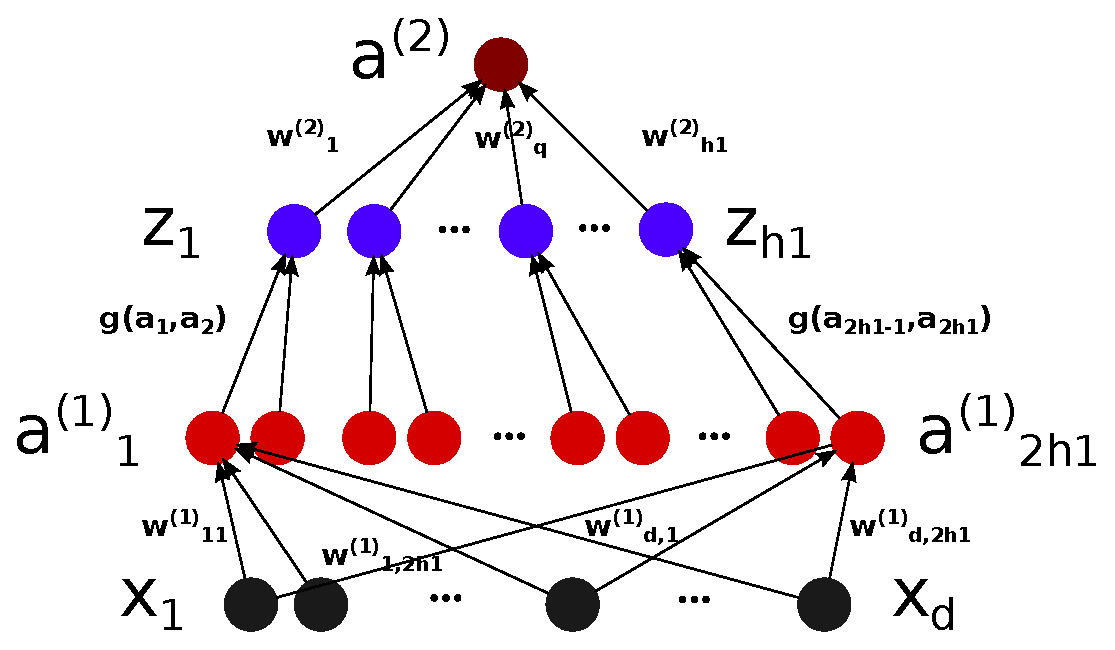
\includegraphics[width=.8\textwidth]{mlp/mlp.eps}
	\label{mlp}
	\caption{dfdf}
\end{figure}

\paragraph{Early stopping}
Evaluate empirical error $\hat{R}(\hat{f};\mathcal{D}_V)$ for validation set $\mathcal{D}_V$ along-side the training-error $\hat{R}(\hat{f};\mathcal{D}_T)$while training the MLP on $\mathcal{D}_T$. Stop at the training at the epoch where the validation error stops decreasing and starts increasing. 
\subsubsection{Parameters for subtasks}

\subsubsection{Examples of overfitting}

\section{Results}
\section{Support Vector Machine}

\subsection{Methods}

\subsubsection{Treatment of Data}

\paragraph{Splitting}

\paragraph{Preprocessing}

\subsubsection{SVM setup}
include all implementation details including choice of C and of $\tao$\\
evaluate 10-fold CV scores for all combinations of the matrix

\subsection{Results}

\end{document}

